\documentclass[11pt, a4paper, pdf]{article}
\newcounter{minitocdepth}
\newcounter{chapter}
\newcommand{\chaptername}{}

%\include{estil-llibre}
\usepackage{iesbbook}

\renewcommand{\hot}[1][]{
	\ifthenelse{\equal{#1}{}}{$\mathbf{\bigstar}$ \underline{\textbf{LLIBRE}}: }{\myrepeat{#1}{$\mathbf{\bigstar}$}}
}
 \renewcommand{\normalsize}{\fontsize{10.5}{11.2}\selectfont}
 
 \fancypagestyle{blocfancy}{
 	\pagestyle{fancy}% Duplicate fancy page style
 	\fancyhead{} % clear all header fields
 	\fancyhead[RE,LO]{\textit{IES Binissalem. Apunts de còniques}}
 	\fancyhead[LE,RO]{\bfseries\large\thepage}
 }
 
\begin{document}
\pagestyle{blocfancy}
\setcounter{myenumi}{0}
 
 \begin{center}
 {\Large  \textbf{Apunts de còniques}}
 \end{center}
 
 \vspace{-0.5cm}
 
\section{Les còniques com a seccions d'una superfície cònica}
\begin{theorybox}
	\begin{multicols}{4}
		\scriptsize
		Si el pla que talla a la superfície cònica és perpendicular a l'eix, la secció és una \textbf{circumferència}.
		\begin{center}
			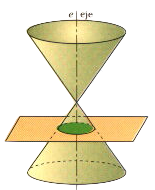
\includegraphics[height=3.cm]{img2/circumferencia.png}
		\end{center}
		
		Si inclinam el pla de manera que sigui oblic amb l'eix i talli a totes les generatrius, la secció és una \textbf{el·lipse}.
		\begin{center}
			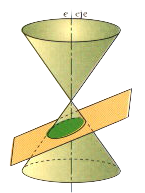
\includegraphics[height=3.cm]{img2/ellipse.png}
		\end{center}
		
		Si continuam inclinant el pla de manera que sigui paral·lel a una generatriu, resulta una \textbf{paràbola}.
		\begin{center}
			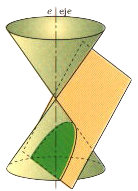
\includegraphics[height=3.cm]{img2/parabola.png}
		\end{center}
		
		Finalment, si inclinam encara més el pla, obtenim una figura amb dues branques que s'anomena \textbf{hipèrbola}.
		\begin{center}
			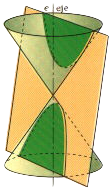
\includegraphics[height=3.cm]{img2/hiperbola.png}
		\end{center}
		
	\end{multicols}	
\end{theorybox}



%%%%%%%%%%%%%%%%%%%%%%%%%%%%%%%%%%%%%%%%%%%%%%%%%%%%%%%%%%%%%%%%%%%%%%%%%%%%%%%%%%%%%%%%%%%%%%%%%%%%%%%%%%%%%%%%%%%%%%%%%%%%%%%

\section{La circumferència}

\begin{theorybox}
	\begin{wrapfigure}{R}{0.3\textwidth} 
		\vspace{-0.5cm}
		\begin{center}
			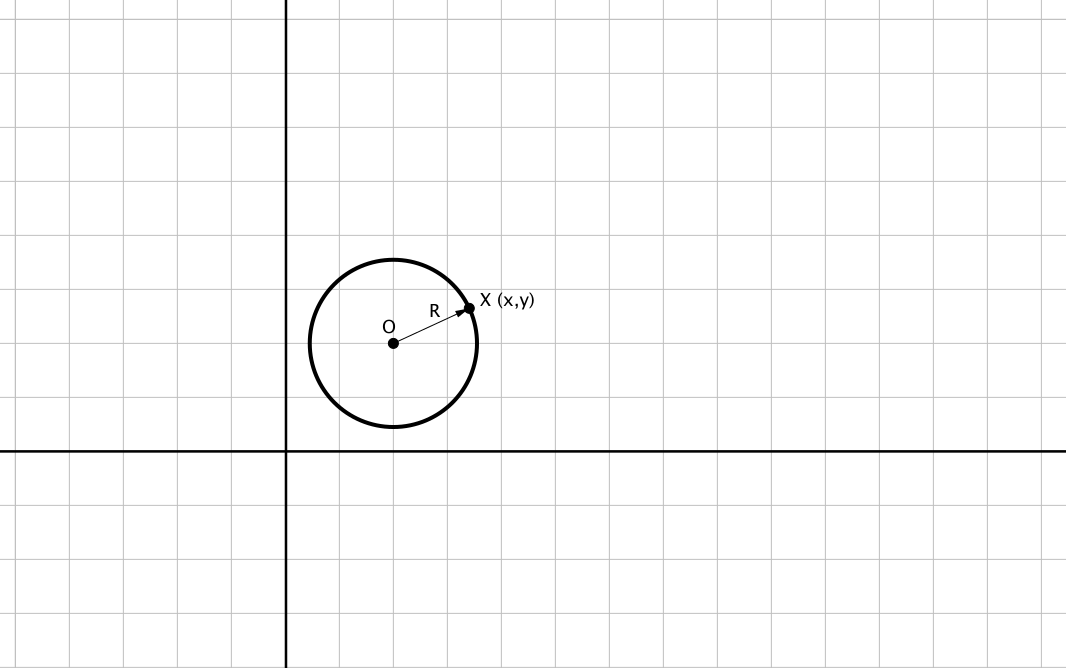
\includegraphics[width=0.26\textwidth]{img2/circ2.png}
		\end{center}
	\end{wrapfigure}

\textbf{És defineix una circumferència com el lloc geomètric de tots els punts del pla
	que equidisten d'un punt anomenat centre.
}
	
	L'equació canònica d'una circumferència de radi $R$ i centre el punt $O(x_0, y_0)$ és:
	\begin{equation}
	\label{eq:circ-canonica}
	(x-x_0)^2+(y-y_0)^2=R^2
	\end{equation}
	
	Si efectuam els quadrats en l'equació (\ref{eq:circ-canonica}) obtindrem l'expressió general de la circumferència:
	\begin{equation}
	\label{eq:circ-genreal}
	x^2+y^2+Ax+By+C=0
	\end{equation}
	essent $A=-2x_0$, $B=-2y_0$, $C=x_0^2+y_0^2-R^2$. És important notar que només serà possible formar una circumferència si $x_0^2+y_0^2-C > 0$.
	
\end{theorybox}

\begin{resolt}[Exemple]{Calcula l'equació canònica i general de la circumferència de centre $O(3,0)$ i que passa pel punt $P(5,2)$.}
	En primer lloc calculam el radi $R=dist(O, P)=\sqrt{(5-3)^2+(2-0)^2}=\sqrt{8}$. L'equació canònica és $(x-3)^2+(y-0)^2=8$. Si efectuam els quadrats, trobam l'equació general: $x^2+y^2-6x+1=0$. 
\end{resolt}
\vspace{-0.75cm}
\begin{resolt}{Donada la circumferència d'equació $x^2+y^2+4x-10y+13=0$ troba el seu centre i radi.}
	De l'equació general identificam els coeficients $A=4$, $B=-10$ i $C=13$. Si utilitzam les relacions:  $4=-2x_0$,  $-10=-2y_0$ automàticament tenim el centre $x_0=-2$ i $y_0=5$. Per trobar el radi utilitzam la darrera relació: $13=(-2)^2+5^2-R^2$. Si d'aquí aïllam $R$ trobam $R=4$. Aquesta circumferència té d'equació canònica $(x+2)^2+(y-5)^2=4^2$.	
\end{resolt}

\begin{mylist}
	
	\item  Calcula l'equació general de la circumferència que passa pel punt \textit{A}=(1, 1) i té per centre a  $C$=($-$1, 3)
	
	\item  Comprova que $x^{2} -2x+y^{2} =0$ és l'equació d'una circumferència. Troba'n el centre i el radi. Dibuixa-la.
	
\end{mylist}

%%%%%%%%%%%%%%%%%%%%%%%%%%%%%%%%%%%%%%%%%%%%%%%%%%%%%%%%%%%%%%%%%%%%%%%%%%%%%%%%%%%%%%%%%%%%%%%%%%%%%%%%%%%%%%%%%%%%%%%%%%%%%%%
\section{L'el·lipse}
\begin{theorybox}
	
	És defineix l'el·lipse com el lloc geomètric de tots els punts del pla
	tals que la \textbf{suma de les distàncies} a dos punts fixos anomenats focus es manté constant.
	
	L'equació canònica d'una el·lipse de semieixos $a$ i $b$ i centre el punt $O(x_0, y_0)$ és:
	\begin{wrapfigure}{R}{0.3\textwidth} 
		\vspace{-1cm}
		\begin{center}
			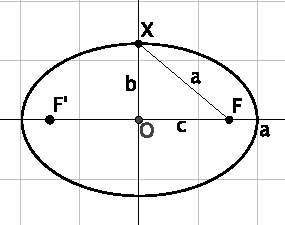
\includegraphics[width=0.28\textwidth]{img2/ellip2.png}
		\end{center}
		\vspace{-1cm}
	\end{wrapfigure}
	\begin{equation}
	\label{eq:ellipse-canonica}
	\frac{(x-x_0)^2}{a^2}+\frac{(y-y_0)^2}{b^2}=1
	\end{equation}
	
	
	Quan els \textbf{semieixos} d'una el·lipse són iguals $a=b=R$, trobam l'equació (\ref{eq:circ-canonica}) de la circumferència.
	
	Els vèrtexs estan situats en els punts $(x_0-a, y_0)$, $(x_0+a, y_0)$, $(x_0, y_0-b)$, $(x_0, y_0+b)$. Els focus els trobam en els punts $F(x_0+c, y_0)$ i $F'(x_0-c,y_0)$.
	
	Definim $c$ com la \textbf{semi-distància focal}. A qualsevol el·lipse 
	
	\[ \boxed{a^2=b^2+c^2} \]
	
	Una mesura de quan estirada és una el·lipse ens ho dóna \textbf{l'excentricitat} $\boxed{e=\frac{c}{a}}$. Per una el·lipse es compleix que $0<e<1$. Quan $e \rightarrow 0$ és pràcticament una circumferència i $e \rightarrow 1$ s'assembla a un ``spaghetti''. 
	
\end{theorybox}


\begin{resolt}[E]{Calcula l'equació de l'el·lipse sabent que té centre a $O(0,0)$, té semiex major 8 i que un dels focus és al punt $F(3,0)$. Calcula la seva excentricitat. }
	Si el centre és $(0,0)$, l'equació canònica es redueix a $\frac{x^2}{a^2}+\frac{y^2}{b^2}=1$. Una de les dades és que el semieix major val $a=8$ i que la semi-distància focal és $c=3$. Falta trobar $b=\sqrt{a^2-c^2}=\sqrt{55}$. L'equació és: $\frac{x^2}{64}+\frac{y^2}{55}=1$.
	
	L'excentricitat és $e=c/a = 3/8 = 0.375 $, obviament menor que 1.
	
\end{resolt}
\vspace{-0.75cm}
\begin{resolt}{Donada l'equació de l'el·lipse  $\frac{x^2}{9}+y^2=1$, troba la posició dels seus focus i dels vèrtexs. Troba la seva excentricitat. }
	
	
	En primer lloc veim que el centre és el punt $(0,0)$. El semieix major val $a=\sqrt{9}=3$ i el semi-eix menor $b=1$. La semi-distància focal es troba de $c=\sqrt{a^2-b^2}=\sqrt{8}$. 
	
	Els vèrtexs estan a $(-3,0)$; $(3,0)$; $(0,1)$; $(0,-1)$. Els dos focus es troben a $F'(-\sqrt{8},0)$ i $F(\sqrt{8},0)$.  
	
	L'excentricitat és $e=c/a = \sqrt{8}/3 = 0.943$ propera a 1, cosa que ens indica que és bastant allargada.
	
\end{resolt}

\begin{mylist}
	\item Una el·lipse té focus en (1, 2) i en (5, 2) i passa pel punt (0, 2). Calcula la seva equació i dibuixa-la. Quant val l'excentricitat?
	
	\item Calcula el centre, semi-eixos, focus i excentricitat de l'el·lipse  $\dfrac{\left(x+1\right)^{2} }{9} +\dfrac{\left(y-1\right)^{2} }{4} =1$.
\end{mylist}
%%%%%%%%%%%%%%%%%%%%%%%%%%%%%%%%%%%%%%%%%%%%%%%%%%%%%%%%%%%%%%%%%%%%%%%%%%%%%%%%%%%%%%%%%%%%%%%%%%%%%%%%%%%%%%%%%%%%%%%%%%%%%%%
\newpage
\section{La hipèrbola}
\begin{theorybox}
	
	És defineix la hipèrbola com el lloc geomètric de tots els punts del pla
	tals que la \textbf{diferència de les distàncies} a dos punts fixos anomenats focus es manté constant.
	
	L'equació canònica d'una hipèrbola de \textbf{semieixos $a$ i $b$} i centre el punt $(x_0, y_0)$ és:
	\begin{wrapfigure}{R}{0.34\textwidth} 
		\vspace{-1cm}
		\begin{center}
			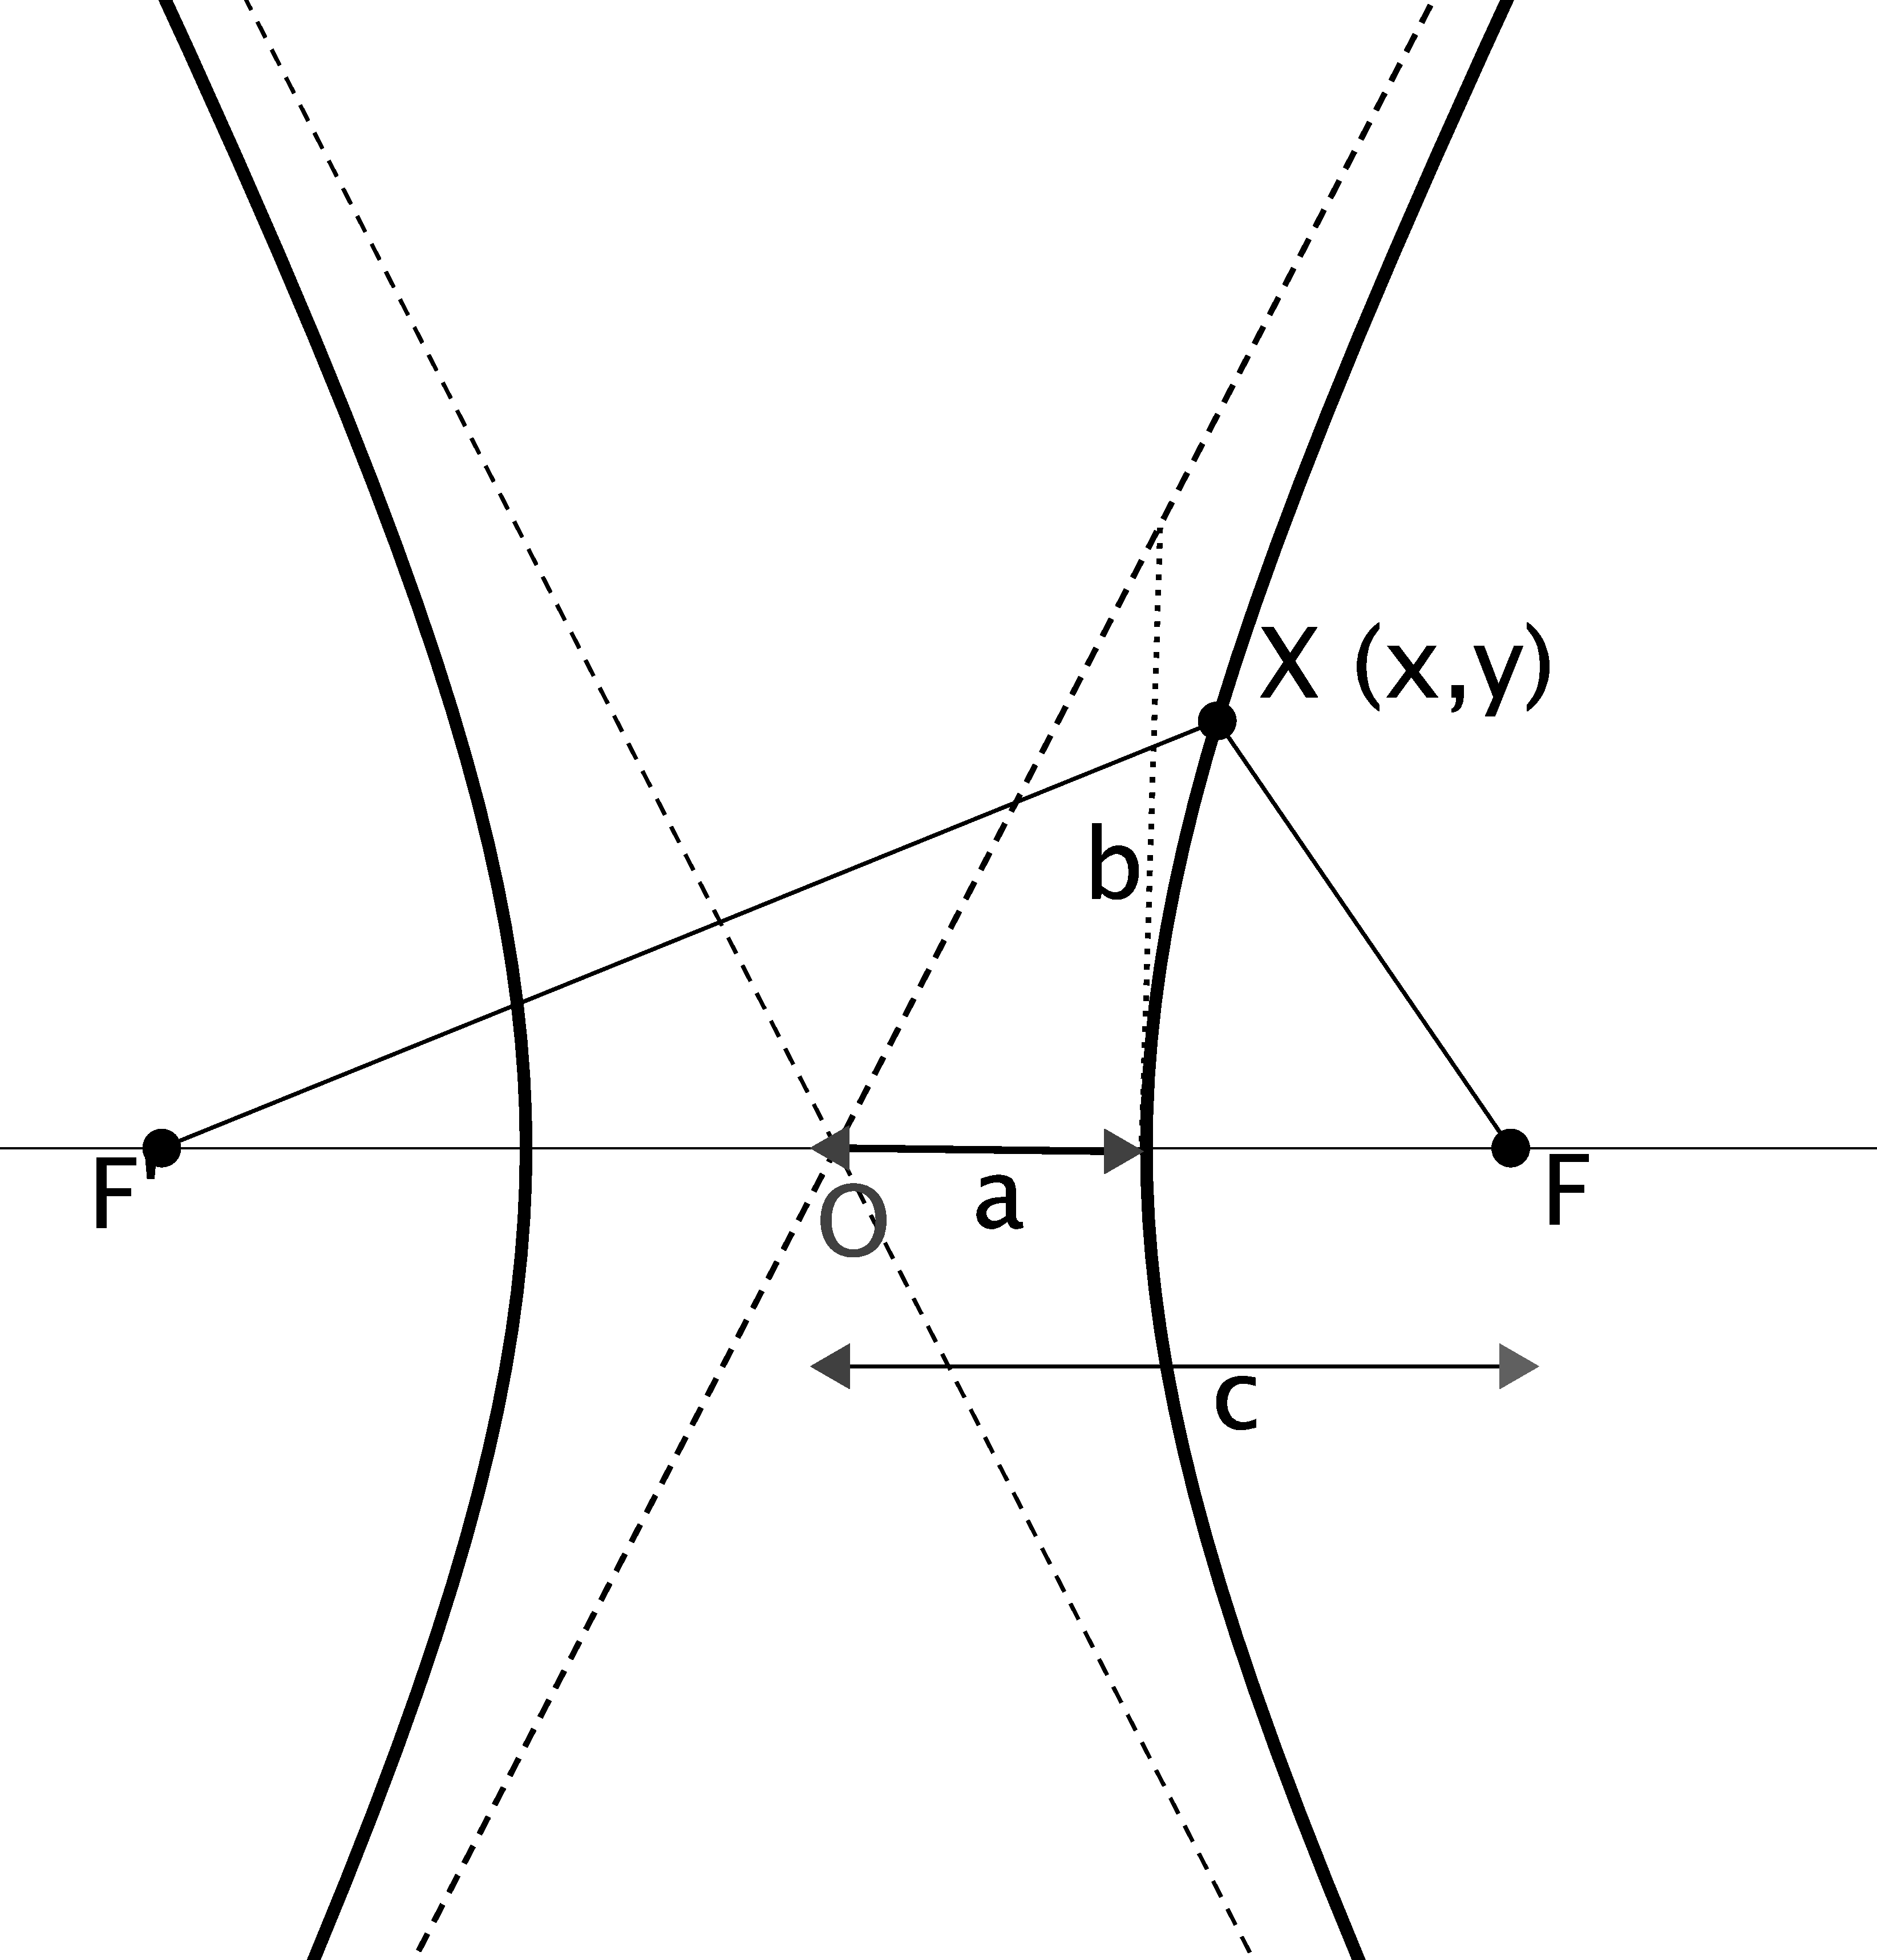
\includegraphics[width=0.32\textwidth]{img2/hiperb2.png}
		\end{center}
		\vspace{-1cm}
	\end{wrapfigure}
	\begin{equation}
	\label{eq:hiperbola-canonica}
	\frac{(x-x_0)^2}{a^2}-\frac{(y-y_0)^2}{b^2}=1
	\end{equation} 
	
	Els vèrtexs estan situats en els punts $(x_0-a, y_0)$, $(x_0+a, y_0)$. Els focus els trobam en els punts $F(x_0+c, y_0)$ i $F'(x_0-c,y_0)$.
	
	Definim $c$ com la \textbf{semi-distància focal}. A qualsevol hipèrbola es compleix que  \fbox{$c^2=a^2+b^2$}. \textbf{L'excentricitat} $e=\frac{c}{a}$ per una hipèrbola compleix que $e>1$. 
	
	
	
	Les dues branques d'una hipèrbola s'acosten a dues \textbf{asímptotes obliqües} que tenen com equacions $\boxed{y=\pm \frac{b}{a} x}$. 
	
	Si $a=b$, es diu \textbf{hipèrbola equilàtera} i es compleix que les dues asímptotes formen un angle recte. Si prenem les asímptotes com a eixos, l'equació de la hipèrbola equilàtera es trasforma en $xy=k$.
\end{theorybox}

\begin{resolt}[E]{Calcula l'equació de la hipèrbola sabent que té centre a $O(0,0)$, semi-distància focal 6 i excentricitat 2. Calcula les seves asímptotes. Representa-ho tot gràficament.}
	\begin{wrapfigure}{R}{0.34\textwidth} 
		\vspace{-0.5cm}
		\begin{center}
			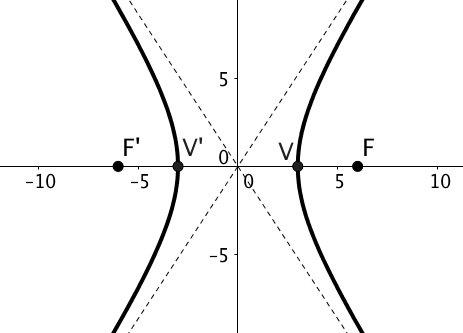
\includegraphics[width=0.3\textwidth]{img2/exem-h2.png}
		\end{center}
	\end{wrapfigure}
	
	Si el centre és $(0,0)$, l'equació canònica es redueix a \linebreak $\frac{x^2}{a^2}-\frac{y^2}{b^2}=1$. Una de les dades és que el semi-distància focal val $c=6$ i que l'excentricitat és $e=2$. Sabem que $e=c/a$, i d'aquí aïllam el semieix major  $a=c/e=6/2=3$. Falta trobar el semi-eix menor $b=\sqrt{c^2-a^2}=\sqrt{27}$. L'equació és: $\frac{x^2}{9}-\frac{y^2}{27}=1$.
	
	Les asímptotes són $y=\pm \frac{\sqrt{27}}{6}x$.
\end{resolt}
\begin{resolt}{ Donada l'equació de la hipèrbola  $x^2-y^2=9$, troba la posició dels seus focus i dels vèrtexs. Calcula la seva excentricitat. }
	
	Es tracta d'una hipèrbola equilàtera $a=b=3$. El centre és el punt $(0,0)$. La semi-distància focal es troba de $c=\sqrt{a^2+b^2}=\sqrt{18}=3\sqrt{2}$. 
	
	Els vèrtexs estan a $(-3,0)$; $(3,0)$. Els dos focus es troben a $F'(-3\sqrt{2},0)$ i $F(3\sqrt{2},0)$.  
	
	L'excentricitat és $e=c/a = 3\sqrt{2}/3 = \sqrt{2}\approx 1.41$.
\end{resolt}

\begin{mylist}
	\item Donada la hipèrbola $\dfrac{\left(x-1\right)^{2}}{16} -\dfrac{{y}^{2}}{9} =1$, calcula el centre, els seus focus, asímptotes i la seva excentricitat.
	
	
	\item  Calcula l'equació de la hipèrbola equilàtera que té per focus $\left(2,\; 2\right)$ i $\left(-2,\quad 2\right)$, així com els seus paràmetres \textit{a}  i  \textit{b} i la seva excentricitat. Dibuixa-la.
	
\end{mylist}

%%%%%%%%%%%%%%%%%%%%%%%%%%%%%%%%%%%%%%%%%%%%%%%%%%%%%%%%%%%%%%%%%%%%%%%%%%%%%%%%%%%%%%%%%%%%%%%%%%%%%%%%%%%%%%%%%%%%%%%%%%%%%%%
\section{La paràbola}

\begin{theorybox}
	\begin{wrapfigure}{R}{0.3\textwidth} 
		\vspace{-0.5cm}
		\begin{center}
			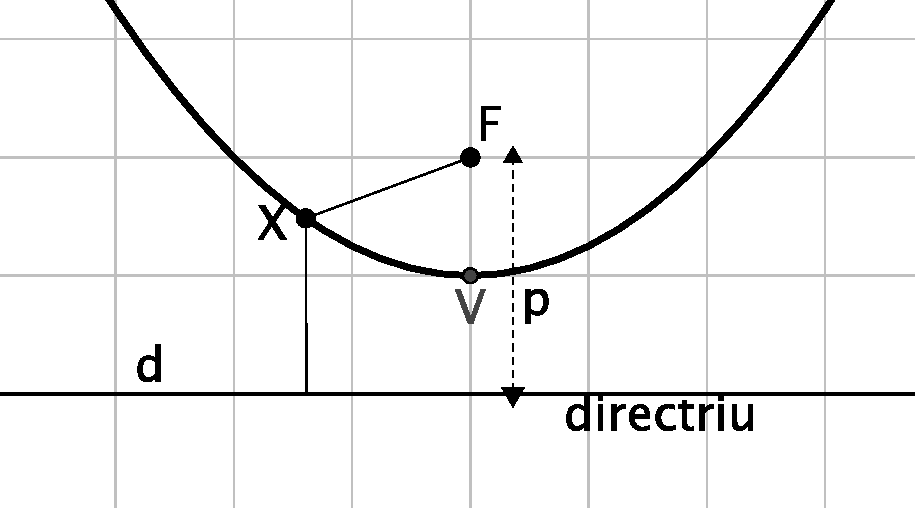
\includegraphics[width=0.28\textwidth]{img2/parab2.png}
			\vspace{-1cm}
		\end{center}
	\end{wrapfigure}
	És defineix la paràbola com el lloc geomètric de tots els punts del pla
	tals que la distància a un punt fix anomenat \textbf{focus és igual a la distància a una recta anomenada directriu}.
	
	Si anomenam $p$ la distància entre el Focus i la directriu, i suposam que la directriu és la recta horitzontal $y=-p/2$ i el focus és al punt $F(0, p/2)$, trobam la \textbf{paràbola vertical}:
	\begin{equation}
	\label{eq:parabola-v}
	y=\frac{1}{2p}x^2
	\end{equation} 
	Aquesta paràbola té el vèrtex en $V(0,0)$. Si desplaçam el vèrtex al punt $V(x_0,y_0)$, l'equació canviaria a $y-y_0=\dfrac{1}{2p}(x-x_0)^2$.
	
	Si la directriu és la recta horitzontal $x=-p/2$ i el focus és al punt $F(p/2, 0)$, trobam la \textbf{paràbola horitzontal}:
	\begin{equation}
	\label{eq:parabola-h}
	x = \frac{1}{2p}y^2
	\end{equation} 
	Aquesta paràbola també té el vèrtex en $V(0,0)$.
	
	Totes les paràboles tenen \textbf{excentricitat} $e=1$.
	
\end{theorybox}


\begin{resolt}[E]{ Calcula l'equació de la paràbola que té el focus al punt $F(5,0)$ i com directriu la recta $x=-5$. Representa-la gràficament.
	}
	\begin{wrapfigure}{R}{0.3\textwidth} 
		\vspace{-0.5cm}
		\begin{center}
			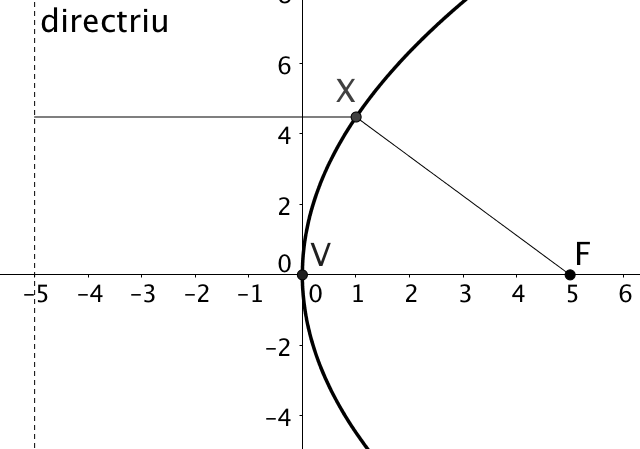
\includegraphics[width=0.28\textwidth]{img2/exem-p1.png}
		\end{center}
	\end{wrapfigure}
	
	
	
	Es tracta d'una paràbola horitzontal amb $p=10$. El vèrtex és el punt $(0,0)$.  L'equació és $x=\frac{1}{20}y^2$.
	
	\vspace*{1.5cm}
	
\end{resolt}
\begin{resolt}{Considera la paràbola  $y=-2 x^2 + 1$, troba la posició del seu focus, el vèrtex i l'equació de la directriu. Representa gràficament la situació.}
	\begin{wrapfigure}{R}{0.3\textwidth} 
		\vspace{-0.5cm}
		\begin{center}
			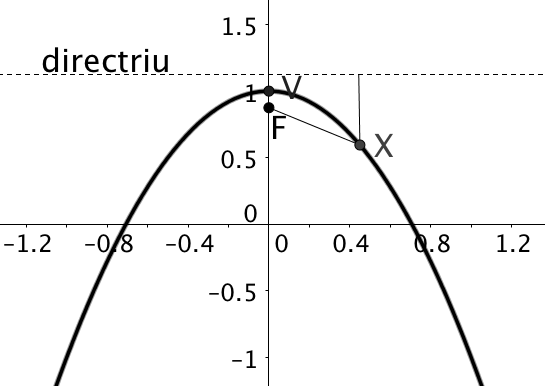
\includegraphics[width=0.28\textwidth]{img2/exem-p2.png}
		\end{center}
	\end{wrapfigure}
	
	
	Es tracta d'una paràbola vertical. El vèrtex és el punt $V(0, 1)$. La distància entre el focus i la directriu és $-2=\frac{1}{2p}$, és a dir, $p=-1/4$. El signe negatiu significa que la directriu està per damunt el focus, és a dir, la paràbola és convexa. La directriu és la recta horitzontal $y= 1+1/8=9/8$ i el focus es troba a $F(0,7/8)$. 
	
	
\end{resolt}
 
 \vspace{1cm}

\begin{mylist}
	\item Calcula l'equació de la paràbola amb focus $F(3,0)$ i directriu la recta $x=-3$.
	
	\item Calcula el vèrtex, focus i directriu de la paràbola $4y=(x-3)^2$.
\end{mylist}

 
\end{document}